%
% File naaclhlt2018.tex

\documentclass[11pt,a4paper]{article}
\usepackage[hyperref]{naaclhlt2018}
\usepackage{times}
\usepackage{latexsym}
\usepackage{tikz}
\usepackage[warn]{textcomp}

\usepackage{url}

\usepackage{etoolbox}
\makeatletter
\patchcmd\@combinedblfloats{\box\@outputbox}{\unvbox\@outputbox}{}{%
   \errmessage{\noexpand\@combinedblfloats could not be patched}%
}%
 \makeatother

%\aclfinalcopy % Uncomment this line for the final submission
%\def\aclpaperid{***} %  Enter the acl Paper ID here

%\setlength\titlebox{5cm}
% You can expand the titlebox if you need extra space
% to show all the authors. Please do not make the titlebox
% smaller than 5cm (the original size); we will check this
% in the camera-ready version and ask you to change it back.

\title{Deep Multitask Learning for Transition-Based DAG Parsing}

\author{Daniel Hershcovich$^{1,2}$ \\
  \\\And
  Omri Abend$^2$ \\
  $^1$The Edmond and Lily Safra Center for Brain Sciences \\
  $^2$School of Computer Science and Engineering \\
  Hebrew University of Jerusalem \\
  \texttt{\{danielh,oabend,arir\}@cs.huji.ac.il}
  \\\And
  Ari Rappoport$^2$
}

\date{}

\begin{document}
\maketitle
\begin{abstract}
  Semantic representation schemes differ in many ways, but we show
  how they are similar and how this similarity can be exploited to
  improve parsing each of them.
  We train a general transition-based parser in a multitask setting
  and show improvements on multiple semantic parsing tasks.
\end{abstract}

\section{Introduction}\label{sec:introduction}

Following increased interest in semantic representation,
recent developments in natural language processing have focused on semantic parsing,
including frame-semantic parsing \cite{gildea2002automatic,swayamdipta2017frame,ringgaard2017sling},
Abstract Meaning Representation parsing \cite{damonte-17,11099},
Semantic Dependency Parsing \cite{P17-1186}, and
Universal Conceptual Cognitive Annotation parsing \cite{hershcovich2017a}, among others.
In parallel, Universal Dependency parsers \cite{dozat2016deep} are improving,
learning syntactic structure in a language-universal way.

While each of these representation schemes has its own set of distinctions it focuses on,
much of the semantic content is shared between many of them \cite{abend2017state}.
Given the success of multitask learning models in various tasks
\cite{collobert2008unified,luong2015multi,ruder2017overview}
including parsing specifically
\cite{Zhang2016StackpropagationIR,P17-1186,swayamdipta2017frame,guo2016exploiting}
and multilingual parsing \cite{TACL892},
we propose a multitask transition-based semantic parser.


\section{Tasks}\label{sec:tasks}

We consider four target representations in this work: UCCA, AMR, SDP and UD.

\subsection{Universal Conceptual Cognitive Annotation}\label{sec:ucca}

UCCA graphs are labeled, directed acyclic graphs (DAGs),
whose leaves correspond to the tokens of
the text. A node (or {\it unit}) corresponds to a terminal or
to several terminals (not necessarily contiguous) viewed as a
single entity according to semantic or cognitive considerations.
Edges bear a category, indicating the role of the sub-unit in the parent relation.

UCCA is a multi-layered representation, where each layer corresponds
to a ``module'' of semantic distinctions.
UCCA's \textit{foundational layer}, targeted in this paper, covers the predicate-argument
structure evoked by predicates of all grammatical categories
(verbal, nominal, adjectival and others), the inter-relations between them,
and other major linguistic phenomena such as coordination and multi-word expressions.
The layer's basic notion is the \textit{scene},
describing a state, action, movement or some other relation that evolves in time.
Each scene contains one main relation (marked as either a Process or a State),
as well as one or more Participants.
Further categories account for inter-scene relations and the internal structure of
complex arguments and relations (e.g. coordination, multi-word expressions and modification).

One incoming edge for each non-root node is marked as \textit{primary},
and the rest (mostly used for implicit relations and arguments) as \textit{remote} edges,
a distinction made by the annotator.
The primary edges thus form a tree structure, whereas the remote edges enable reentrancy,
forming a DAG.

\subsection{Abstract Meaning Representation}\label{sec:amr}

Abstract Meaning Representation \cite[AMR; ][]{banarescu2013abstract}
is a semantic representation for natural
language that embeds annotations related
to traditional tasks such as named entity
recognition, semantic role labeling, word
sense disambiguation and co-reference
resolution.

AMRs are rooted and directed
graphs with node and edge labels.
For most sentences in our dataset, the
AMR graph is a directed acyclic graph (DAG),
with a few specific cases where cycles are permitted.
These cases are rare, and for the purpose of
this paper, we consider AMR as DAGs.

\subsection{Semantic Dependency Parsing}\label{sec:sdp}

First defined in a SemEval 2014 shared task
\cite{oepen2014semeval}, and then extended by \citet{oepen2015semeval},
the broad-coverage semantic dependency parsing (SDP) task is centered around three
semantic formalisms whose annotations have been
converted into bilexical dependencies. The formalisms come
from varied linguistic traditions, but all three aim
to capture predicate-argument relations between
content-bearing words in a sentence.
While at first glance similar to syntactic dependencies,
semantic dependencies have distinct
goals and characteristics, more akin to semantic
role labeling \cite[SRL; ][]{gildea2002automatic} or
AMR. They abstract over different
syntactic realizations of the same or similar meaning.
Conversely, they attempt to distinguish
between different senses even when realized
in similar syntactic forms.
Structurally, they are labeled directed graphs
whose vertices are tokens in the sentence.
Their arc labels encode broadly-applicable semantic relations rather than being tailored
to any specific downstream application or
ontology.
They are not necessarily trees, because
a token may be an argument of more than one
predicate. Their analyses may optionally leave out non-content-bearing
tokens, such as punctuation or the infinitival ``to,'' or prepositions that simply mark
the type of relation holding between other words.
But when restricted to content-bearing tokens (including
adjectives, adverbs, etc.), the subgraph
is connected. In this sense, SDP provides a
whole-sentence analysis. This is in contrast to
PropBank-style SRL, which gives an analysis of
only verbal and nominal predicates \cite{Palmer:05}.
Semantic dependency graphs also tend to
have higher levels of nonprojectivity than syntactic
trees \cite{oepen2014semeval}. Sentences with
graphs containing cycles have been removed from
the dataset by the organizers, so all remaining
graphs are directed acyclic graphs.

We consider one of the three formalisms used in the SemEval shared task:
the DM (DELPH-IN MRS) representation, which comes
from DeepBank \cite{flickinger2012deepbank},
manually-corrected parses from the LinGO
English Resource Grammar \cite{copestake2000open}.
LinGO is a head-driven phrase
structure grammar \cite[HPSG; ][]{pollard1994head}
with minimal recursion semantics \cite{copestake2005minimal}.

\subsection{Universal Dependencies}\label{sec:ud}

In recent years, the Universal Dependencies
(UD) representation \cite{nivre2016universal,11234/1-2515} has become
the dominant dependency representation for
annotating treebanks in a large variety of languages.
The goal of the UD project is to provide
guidelines for cross-linguistically consistent treebank
annotations for as many languages as possible.



\section{Transition-Based Universal Parser}\label{sec:model}

To create a parser that can handle multiple tasks (annotation schemes),
we extend TUPA \cite{hershcovich2017a}, a transition-based parser for UCCA,
to allow training and testing it on any DAG structure.
To that end, we propose a conversion algorithm for each scheme,
to convert it into a unified DAG format (see Subsection~\ref{sec:conversion}).

Similarly to \citet{hershcovich2017a}, we use a transition-based parser
with a general transition system that allows parsing any DAG structure.
To demonstrate its applicability, we apply the parser to the four datasets
in a single-task setting.
The transition system supports reentrancies, discontinuities and non-terminal nodes.
In addition, we define a transition for labeling nodes, to support AMR parsing.

Transition-based parsers \cite{Nivre03anefficient} scan the text from start to end,
and create the parse incrementally by applying a \textit{transition}
at each step to the parser's state,
defined using three data structures: a buffer $B$ of tokens and nodes to be processed,
a stack $S$ of nodes currently being processed,
and a graph $G=(V,E,\ell)$ of constructed nodes and edges,
where $V$ is the set of \emph{nodes}, $E$ is the set of \emph{edges},
and $\ell : E \to L$ is the \emph{label} function, $L$ being the set of possible labels.
Some states are marked as \textit{terminal}, meaning that $G$ is the final output.
A classifier is used at each step to select the next transition based on features
encoding the parser's current state.
During training, an oracle creates training instances for the classifier,
based on gold-standard annotations.


\subsection{Transition Set}\label{sec:transition_set}
Given a sequence of tokens $w_1, \ldots, w_n$, we predict a graph $G$ over the sequence.
Parsing starts with a single node on the stack (an artificial root node), and the input tokens
in the buffer.

The transitions used in \citet{hershcovich2017a} are
the standard \textsc{Shift} and \textsc{Reduce} operations,
\textsc{Node$_X$} for creating a new non-terminal node and an $X$-labeled edge,
\textsc{Left-Edge$_X$} and \textsc{Right-Edge$_X$} to create a new primary $X$-labeled edge,
\textsc{Left-Remote$_X$} and \textsc{Right-Remote$_X$} to create a new remote $X$-labeled edge,
\textsc{Swap} to handle discontinuous nodes,
and \textsc{Finish} to mark the state as terminal.

In addition, we add the \textsc{Implicit} transition, creating a new non-terminal
node as a \textit{child} of the current stack top rather than as its parent.
Although UCCA (as well as AMR) contains implicit units, that is, units without
any terminals as descendents,
the standard evaluation for UCCA \cite{hershcovich2017a} is span-based and
ignores these nodes.
For this reason we do not include this transition when parsing UCCA.
However, for AMR we do include it, as AMRs contain unaligned concepts,
which correspond to implicit nodes in the unified format.

For parsing AMR, we also use a \textsc{Label$_i$} transition for $i=1,2$,
adding a label for the $i$th node from the top of the stack
(i.e., stack top or one node to its left).
To keep the overall number of transitions manageable,
the node label itself is not part of the transition's identity,
instead being selected by a separate classifier.

\subsection{Classifier}\label{sec:classifier}
Following \citet{hershcovich2017a}, we experiment with two different models for the parser:
a linear classifier with sparse features, trained with the averaged structured perceptron algorithm
\cite{Coll:04} and \textsc{MinUpdate} \cite{goldberg2011learning},
and a bidirectional LSTM with dense embedding features,
combined with a feedforward network.
We experiment with the softmax loss funnction and also max-margin.
For softmax, we sum over all correct actions.
For max-margin, we subtract the highest-scoring incorrect action score
from the highest-scoring correct action score.

For all classifiers, inference is performed greedily,
and training is done with an oracle that provides a set of all possible labels at a given state
(but only valid transitions may be taken during training).
Hyperparameters are tuned on the development set for each task.

\begin{figure}[t]
   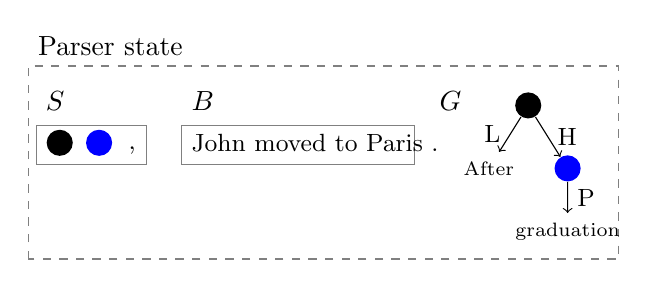
\begin{tikzpicture}[level distance=8mm, sibling distance=1cm]
   \node[anchor=west] at (0,1.5) {Parser state};
   \draw[color=gray,dashed] (0,-1.2) rectangle (7.5,1.25);
   \draw[color=gray] (.1,0) rectangle (1.5,.5);
   \node[anchor=west] at (.1,.8) {$S$};
   \node[fill=black, circle] at (.4,.275) {};
   \node[fill=blue, circle] at (.9,.275) {};
   \node[anchor=west] at (1.15,.175) {\small ,};
   \draw[color=gray] (1.95,0) rectangle (4.9,.5);
   \node[anchor=west] at (1.95,.8) {$B$};
   \node[anchor=west] at (1.95,.275) {\small John moved to Paris .};
   \node[anchor=west] at (5.1,.8) {$G$};
   \node[fill=black, circle] at (6.35,.75) {}
     child {node  {\scriptsize After} edge from parent [->] node[left] {\small L}}
     child {node [fill=blue, circle] {}
     {
       child {node {\scriptsize graduation} edge from parent [->] node[right] {\small P}}
     } edge from parent [->] node[right] {\small H} };
   \end{tikzpicture}
   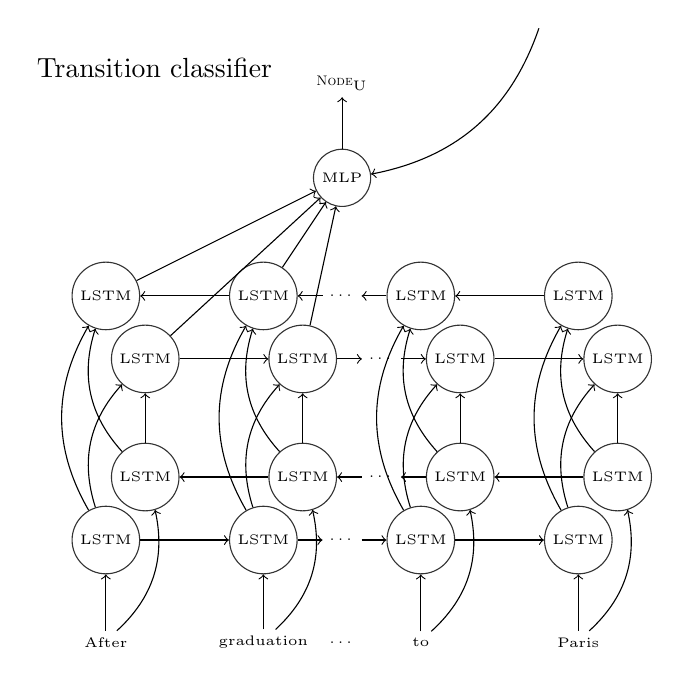
\begin{tikzpicture}[->]
   \node[anchor=west] at (0,6) {Transition classifier};
   \tiny
   \tikzstyle{main}=[circle, minimum size=7mm, draw=black!80, node distance=12mm]
   \foreach \i/\word in {1/{After},3/{graduation},5/{to},7/{Paris}} {
       \node (x\i) at (\i,-1.3) {\word};
       \node[main, fill=white!100] (h\i) at (\i,0) {LSTM};
        \path (x\i) edge (h\i);
       \node[main, fill=white!100] (i\i) at (\i.5,.8) {LSTM};
        \path (x\i) edge [bend right] (i\i);
       \node[main, fill=white!100] (l\i) at (\i.5,2.3) {LSTM};
        \path (h\i) edge [bend left] (l\i);
        \path (i\i) edge (l\i);
       \node[main, fill=white!100] (k\i) at (\i,3.1) {LSTM};
        \path (i\i) edge [bend left] (k\i);
        \path (h\i) edge [bend left] (k\i);
   }
    \node (l4) at (4.5,2.3) {\ldots};
    \node (k4) at (4,3.1) {\ldots};
    \node (i4) at (4.5,.8) {\ldots};
    \node (h4) at (4,0) {\ldots};
    \node (x4) at (4,-1.3) {\ldots};
   \foreach \current/\next in {1/3,3/4,4/5,5/7} {
        \path (i\next) edge (i\current);
        \path (h\current) edge (h\next);
        \path (k\next) edge (k\current);
        \path (l\current) edge (l\next);
   }
    \node[main, fill=white!100] (mlp) at (4,4.6) {MLP};
   \foreach \i in {1,3} {
        \path (l\i) edge (mlp);
        \path (k\i) edge (mlp);
    }
    \coordinate (state) at (6.5,6.5);
    \path (state) edge [bend left] (mlp);
    \node (transition) at (4,5.8) {\textsc{Node}\textsubscript{U}};
    \path (mlp) edge (transition);
   \end{tikzpicture}
   \caption{Illustration of the model.
      Top: parser state (stack, buffer and intermediate graph).
      Bottom: BiLTSM architecture.
      Vector representation for the input tokens is computed
      by two layers of bidirectional LSTMs.
      The vectors for specific tokens are concatenated with
      embedding and numeric features from the parser state
      (for existing edge labels, number of children, etc.),
      and fed into the MLP for selecting the next transition.}
   \label{fig:model}
\end{figure}

We use the same features as \citet{hershcovich2017a}, and for AMR, also node label features according to
previously predicted node labels for node in specific locations in the parser state.
We use sparse features for the linear classifier and embedding features for the NN.

Lemmas, POS tags, syntactic dependency labels and named entities are extracted using spaCy
\cite{spacy2}.\footnote{\url{https://spacy.io}}
We use the categorical cross-entropy objective function and optimize the
NN classifiers with the Adam optimizer \cite{kingma2014adam}.
We use fastText word vectors \cite{bojanowski2016enriching} pretrained over Wikipedia.
The neural network is implemented using DyNet \cite{neubig2017dynet}.\footnote{\url{https://dynet.io}}
Hyperparameter settings are listed in Table~\ref{tab:hyperparams}.

\begin{table}
\begin{tabular}{l|ccc}
& Sparse & NN \\
\hline
\multicolumn{4}{l}{\footnotesize Embedding dimensions} \\
external word & & 100 \\
word & & 200 \\
POS tag & & 20 \\
syntactic dep. & & 10 \\
edge label & & 20 \\
punctuation & & 1 \\
gap & & 3 \\
action & & 3 \\
\hline
\multicolumn{4}{l}{\footnotesize Other parameters} \\
training epochs & 19 & 59 \\
$\textsc{MinUpdate}$ & 5 \\
initial learning rate & 1 & 1 \\
learning rate decay & 0.1 & 1 \\
MLP \#layers & & 2 \\
MLP layer dim. & & 50 \\
LSTM \#layers & & 2 \\
LSTM layer dim. & & 500 \\
word dropout & & 0.2 \\
dropout & & 0.4 \\
weight decay & & $10^{-5}$ \\
mini-batch size & & 100
\end{tabular}
\caption{Hyperparameter settings.\label{tab:hyperparams}}
\end{table}


\subsection{Constraints}

As each annotation framework has different constraints on the allowed graphs,
we declared these constraints separately for each task.
During training and parsing, the constraint set corresponding to the task is
selected and applied to the parser state.

Some constraints are task-specific, while some are generic.
For example, in UCCA, a terminal may only have one parent.
In UD, any node may only have one parent.
In AMR, concept corresponding to PropBank frames may not have core arguments not defined in the frame.

When parsing any scheme, nodes that have already been swapped
should never be swapped again.
Thus, we apply the generic constraints that nodes may be swapped only once.
To implement this constraint efficiently, we define a \textit{swap index}
for each node, which is assigned when the node is created.
At parse start, only the root node and terminals exist.
We assign the root a swap index of 0, and for each terminal, its swap index
is its position in the text (starting at 1).
Whenever a node is created as a result of a \textsc{Node} or \textsc{Implicit}
transition, we assign its swap index to be the mean of the stack top and buffer
head's swap indices.


\subsection{Conversion}\label{sec:conversion}

We develop a conversion algorithm for each scheme,
to convert it into a unified DAG format, similar to the UCCA format.
In this format, the graph is a rooted DAG, and the text token are terminals
(they have no children).
Edges are labeled with \textit{categories}, and
nodes have an optional \textit{label} too, to support AMR.
All edges entering terminals bear the \textsc{Terminal} category.
The graph edges are divided into \textit{primary} and \textit{remote} edges,
where the primary edges form a tree (all nodes have at most one primary parent,
and the root has none).
The remote edges enable reentrancy, and thus together with them the graph
is in general a DAG and not necessarily a tree.
Not all non-terminals must have terminal descendants.
Non-terminals with an empty terminal yield are called \textit{implicit}.

To convert from dependency formats (SDP and UD), we add a pre-terminal for each terminal,
and then simply attach the pre-terminals according to the dependency edges.
In case of reentrancy, an arbitrary parent is marked as primary, and the rest as remote.

The conversion from AMR is more involved:

\paragraph{Alignments.}
Since alignment to the text tokens is not part of the AMR graph,
we introduce the alignments as edges in training.
We use automatically aligned AMR graphs provided in the dataset,
and attach each node with a \textsc{Terminal} edge to each of the terminals it is aligned to.

\paragraph{Sparsity.}
To reduce the number of unique node labels, we use the alignments to introduce
placeholders in the labels.
For example, a node labeled \textit{want-01} aligned to the terminal \textit{wants} will
be instead labeled \textit{\textlangle l\textrangle-01},
where \textit{\textlangle l\textrangle} is a placeholder for the token's lemma.
In this way we reduce the number of node labels from tens of thousands to 7300,
of which 2000 occur only once and are treated as unknown.
In addition, we omit all variable identifiers and instead label nodes directly with their concept.
This is similar to the delexicalization employed by \citet{buys2017oxford}.

Another sparsity issue is with ordinal relations, such as \textit{op1}, \textit{op2}, etc.
Since the order is according to the surface form, the numeric index is redundant and is thus removed.
We keep the numeric suffixes when they are meaningful, e.g. in \textit{ARG0}, \textit{ARG1}, etc.

\paragraph{Names.}



\subsection{Unlabeled parsing}\label{sec:unlabeled}

We extend the parser to support unlabeled parsing by simply removing all labels from
\textsc{Edge}, \textsc{Remote}, \textsc{Node} and \textsc{Implicit} actions output by the oracle.
This results in a much smaller output dimension, but of course only unlabeled evaluation is
meaningful in this case.



\section{Multitask Transition-Based Parsing}\label{sec:multitask}

Since the same model can be applied to different tasks, we also train it jointly on multiple tasks.
In this section we focus on the NN model.
Rather than sharing the whole set of parameters (and getting a mix of action labels as a result),
we share only part of the model.
Specifically, in addition to the task-specific input-encoding bidirectional LSTM,
we use a shared bidirectional LSTM. The outputs of both LSTMs are concatenated and
fed into the task-specific MLP, in a manner similar to \citet{P17-1186}.

Multitask learning is particularly beneficial for improving on tasks with small training data.
As UCCA has a relatively small corpus, we focus on UCCA parsing and treat AMR, SDP and UD parsing
as auxiliary tasks, creating a unified corpus by shuffling all sentences from all datasets together,
but using only the score on the UCCA development set as the criterion for early stopping.

Preliminary experiments showed that simply training the model in this manner yield no improvement
on the UCCA development set, when compared to training on the UCCA corpus alone.
We hypothesized that the auxiliary tasks were actually difficult enough on their own,
and could not provide enough backpropagation signal to the shared parameter set.
We thus decided to use unlabeled parsing for all auxiliary tasks, while still doing labeled UCCA parsing.


\section{Experiments}\label{sec:experiments}

We perform various experiments to evaluate which of the representation schemes benefit each other.
As a baseline, we train the parser separately on each task.

\subsection{Data}\label{sec:data}

For UCCA, we use the English Wikipedia corpus \cite{abend2013universal},
and the \textit{Twenty Thousand Leagues Under the Sea} corpus \cite[20K leagues;][]{sulem2015conceptual},
annotated in English, French and German.
For AMR, we use LDC2016E25, used in SemEval 2017 \cite{may2017semeval}.
For SDP, we use data for the DM target representation from SemEval 2015 \cite{oepen2015semeval}.
For Universal Dependencies, we use UD v2.1 \cite{11234/1-2515}.
Table~\ref{tab:corpora} shows the size of each corpus.

\begin{table}
\begin{tabular}{lcc}
Corpus & \# Tokens & \# Sentences \\
\textbf{UCCA} \\
Wiki & 158433 & 5225 \\
20K Leagues: \\
English & 12339 & 506 \\
French & 12929 & 547 \\
German & 113524 & 4764 \\
\textbf{UD} \\
English & 408466 & 24276 \\
French & 1067840 & 40102 \\
German & 308107 & 16590 \\
\textbf{AMR} \\
LDC2016E25 & 708701 & 39260 \\
\textbf{SDP} \\
SemEval 2015 & 802717 & 35657 \\
\end{tabular}
\caption{Size of each corpus.\label{tab:corpora}}
\end{table}


\subsection{Evaluation}\label{sec:evaluation}

As each scheme has its own evaluation metric, we evaluate them separately.
For UCCA, we evaluate labeled precision, recall and F1 on primary and remote edges.
For UD, we use LAS F1.
For AMR, we use Smatch precision, recall and F1.
For SDP, we use labeled precision, recall and F1.


\subsection{Results}\label{sec:results}




\subsection{Single-task}\label{sec:results_single}

To evaluate the conversion and parsing algorithm on each task, we report the result
of training each 
The results for single-task parsing are shown in Table~\ref{tab:single}.



\begin{table}
\begin{tabular}{llccc}
\textbf{UCCA} & & \textbf{LP} & \textbf{LR} & \textbf{LF} \\
Sparse & \small Primary & 63.4 & 64.3 & 63.8 \\
       & \small Remote & 17 & 14.3 & 15.5 \\
NN & \small Primary & 74.5 & 74.9 & 74.7 \\
       & \small Remote & 49.2 & 50.5 & 49.8 \\
\hline
\textbf{UD} & \small LAS & & & \textbf{F1} \\
Sparse & & & & 64.8 \\
NN & & & & 80.1 \\
\hline
\textbf{AMR} & \small Smatch & \textbf{P} & \textbf{R} & \textbf{F1} \\
Sparse & & 55 & 53.7 & 54.4 \\
NN & & & & 58.2 \\
\hline
\textbf{SDP} & & \textbf{LP} & \textbf{LR} & \textbf{LF} \\
Sparse & & 55 & 51.2 & 53 \\
NN & & 76 & 75.4 & 75.7
\end{tabular}
\caption{Single-task results on the development set for each task.\label{tab:single}}
\end{table}


\subsection{Multitask}\label{sec:results_multi}

The results for multitask parsing are shown in Table~\ref{tab:multi}.

\begin{table}
\begin{tabular}{lccc|ccc}
& \multicolumn{3}{c|}{Primary} & \multicolumn{3}{c}{Remote} \\
& \textbf{LP} & \textbf{LR} & \textbf{LF} & \textbf{LP} & \textbf{LR} & \textbf{LF} \\
\small AMR & 65.8 & 66.8 & 66.3 & 35.6 & 16.5 & 22.6 \\
\small UD & 72.1 & 72.1 & 72.1 & 55 & 42.7 & 48.1 \\
\small SDP & 72.1 & 71.9 & 72 & 53.5 & 48 & 50.6 \\
\small SDP+UD & 71.9 & 71.5 & 71.7 & 46.9 & 31.2 & 37.5 \\
\small AMR+UD & 66.8 & 64.9 & 65.8 & 31.4 & 11.5 & 16.9 \\
\small AMR+SDP & 70.2 & 70.3 & 70.3 & 55.3 & 42.4 & 48 \\
\small all & 71.1 & 71.4 & 71.3 & 43.5 & 38.3 & 40.7
\end{tabular}
\caption{Multitask results on the UCCA Wiki development set.
The UCCA Wiki training set is used in each case, in addition to the training
set for the specified task.\label{tab:multi}}
\end{table}


\subsection{Other languages}\label{sec:other_languages}

To investigate the contribution of multitask training on an even smaller UCCA training set,
we experiment with the French and German \textit{20K Leagues} UCCA corpora.
The results are given in Table~\ref{tab:other_languages}.

\begin{table}
\begin{tabular}{lccc|ccc}
& \multicolumn{3}{c|}{Primary} & \multicolumn{3}{c}{Remote} \\
\textbf{German} & \textbf{LP} & \textbf{LR} & \textbf{LF} & \textbf{LP} & \textbf{LR} & \textbf{LF} \\
UCCA \\
\small Sparse & 67.4 & 65.5 & 66.4 & 24.1 & 2.9 & 5.1 \\
\small NN & 54.2 & 38.4 & 45 & 35 & 17.3 & 23.1 \\
\multicolumn{3}{l}{UCCA + UD} \\
\small NN & 63.8 & 59.6 & 61.6 & 0 & 0 & 0 \\
\hline
\textbf{French} \\
UCCA \\
\small Sparse & 60.8 & 59.2 & 60 & 7.1 & 3.8 & 4.9 \\
\small NN & 100 & 0 & 0 & 100 & 0 & 0 \\
\multicolumn{3}{l}{UCCA + UD} \\
\small NN & 42.2 & 39.2 & 40.6 & 100 & 0 & 0
\end{tabular}
\caption{Single-task and multitask results on the UCCA Wiki development set in German and French.\label{tab:other_languages}}
\end{table}



\section{Related work}\label{sec:related_work}

In general, multitask learning involves optimizing more than one loss function \cite{ruder2017overview}.
However, in our case, the loss function has the same form across all tasks.
The same architecture and inference algorithm are applied to multiple annotation formats and datasets,
and only some of the parameters are shared between them: this is hard parameter sharing.

\cite{swayamdipta2017frame}
\cite{P17-1186}


\section{Discussion}\label{sec:discussion}




\bibliography{references}
\bibliographystyle{acl_natbib}

\end{document}
